We start with an empirical evaluation of the privacy offered by {\sys}'s traffic
shaping.
To evaluate privacy empirically, we first establish the baseline for comparison, which is attacker accuracy, precision, and recall on unmodified (\ie unshaped) traces.
We set up the video service and a video client as two Amazon AWS VMs placed in Oregon and Montreal, respectively.
The client streams the first 5 min of all videos of our video dataset over HTTPS and collects the resulting network packet traces using tcpdump.
We also filter our dataset comprising 10,000 traces and 100 videos to reduce it to a smaller dataset consisting of 40 videos and 4,000 traces.
We evaluate the Beauty and the Burst (BB) model and our TCN-based model with the collected traces using both small and large datasets.
The objective of the models is to determine the corresponding video title for a given trace. 
For each model, we transform each packet trace into a sequence of burst sizes
transmitted within 1s windows.
Therefore, the input to the classifier is a time series representing burst sizes with burst length of 1 second.
We normalize the time series by dividing each burst size by the total size of the corresponding trace.
For each dataset, we use 80\% of traces to train the model and 20\% of traces to test it. 
We train both models for 1000 epochs\footnote{An epoch refers to one complete pass through the entire training dataset during the training.} and report the accuracy, precision, and recall on the test data.
\Cref{tab:attack-performance} represents the result for both models with the two datasets.
Our TCN model outperformes BB model on both datasets. 
Specifically, BB struggles with the larger dataset and its accuracy drops to random guess. 
The presence of residual layers in TCN makes it a better choice for a larger dataset.
\begin{table}[h]
  \centering
  \caption{Attack Performance on unshaped traffic}
  \begin{tabular}{|l|c|c|c|c|}
    \hline
    \textbf{Attack} & \textbf{\# of videos} & \textbf{Accuracy} & \textbf{Precision} & \textbf{Recall} \\ 
    \hline
    \multirow{2}{*}{TCN} & 100 & 0.995 & 0.99 & 0.99 \\ 
                         & 40  & 0.996 & 0.99 & 0.99 \\ 
    \hline
    \multirow{2}{*}{BB}  & 100 & 0.005  & 0.005 & 0.01 \\ 
                         & 40  & 0.61  & 0.49 & 0.63 \\ 
    \hline
  \end{tabular}\label{tab:attack-performance}
\end{table}

Next, we evaluate the efficacy of our differentially-private shaping mechanism against both BB and TCN attacks with the small dataset.
We did not consider the large dataset for this task because the BB model failed to classify the baseline unshaped traffic, making it impossible to see the effectiveness of the DP shaping mechanism for this attack.
The performance of the DP traffic shaping depends on several parameters: the window length $\winlen$, the sensitivity for neighboring streams $\ssens$, the length of the DP measurement interval $\dpintvl$, and the privacy loss $\varepsilon_{\winlen}$.
The privacy of the mechanism, however, is characterized by the privacy loss, $\varepsilon_{\winlen}$
Therefore, we fix values of $\ssens$, $\winlen$, and $\dpintvl$ and measure the accuracy of classifier for varying values of $\varepsilon_{\winlen}$.
As both of attacks fail to perform effectively with small values of $\varepsilon_{\winlen}$ (\ie lower privacy loss), we increment $\varepsilon_{\winlen}$ until one of the attacks yields an accuracy beyond random guessing (\ie $\varepsilon_{\winlen} \in [100, 43000]$).
Our goal is to provide intuition about practical values of $\varepsilon_{\winlen}$ that are sufficient to thwart a side-channel~attack.

We set (i) $\winlen = 5s$ to align with the 5s video segments that comprise the videos, (ii) $\ssens = 1 MB$, which covers 97\% of the video streams in our dataset, and (iii) $\dpintvl = 1s$, which leads to composing the privacy loss over $\varnumupdates = 5$ DP measurements of the buffering queues.

We use 4000 traces of 40 videos, each with 5 minutes duration (\ie small dataset).
For each value of $\varepsilon_{\winlen}$, we transform each unshaped trace into a shaped trace using our simulator to generate a total of 4000 shaped traces.
We train the classifier on 3200 shaped traces and measure the accuracy of the attack model on 800 shaped traces.

\Cref{fig:empirical-privacy} shows the average (markers) and the standard deviation (shaded region) of the accuracy of each classifier over three runs on the shaped traces.
While BB does not perform well for any values of $\varepsilon_{\winlen}$, TCN can be thwarted only for $\varepsilon_{\winlen} < 1000$ with {\sys} (\ns).
The BB and TCN accuracy on unshaped traffic ({\base}) is 0.61 and 0.99, respectively (see \Cref{tab:attack-performance}).
Note that large values of privacy loss (\ie $\varepsilon_{\winlen} \leq 1$) does not provide meaningful theoretical privacy guarantees.
For example, $\varepsilon_{\winlen}=10$ means that given a trace, in the worst-case, the probability that the adversary can correctly identify the video title is $e^{10} \approx 22000$ times larger than the probability that the adversary fails to classify it correctly.
Nonetheless, in practice, we observe that small perturbations with large privacy losses are enough to thwart the state-of-the-art attacks.
This observation highlights the large gap between theoretical guarantees and empirical evaluation of side-channel attacks, which has two important implications: First, the successful mitigation of present attacks by a defense doesn't assure its efficacy against future, more sophisticated attacks.
Second, these findings encourage the development of network side-channel defense mechanisms and their subsequent evaluation based on theoretical privacy considerations, because the empirical evaluation can potentially overestimate the effectiveness of these mechanisms.


\begin{figure}[t]
  \centering
  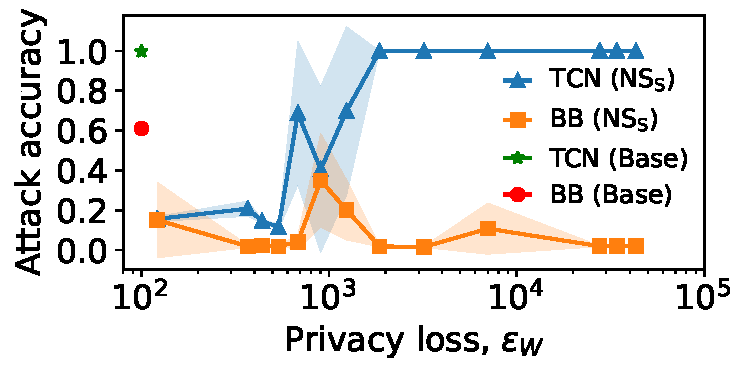
\includegraphics[width=\columnwidth]{plots/accuracy_vs_privacy_loss_video.pdf}
  \caption{Classifier accuracy on shaped traces.
      %    \am{Change label from {\ns} to {\nssim}}
  }
  %\am{How is the blue shaded area going higher than accuracy of 1.0?}\as{The
      %blue shaded area is +-std so it can be larger than one or smaller than
      %zero.}
  \label{fig:empirical-privacy}
\end{figure}